\documentclass[./main.tex]{subfiles}
\graphicspath{{\subfix{./images/}}}

\begin{document}

Arrays are data structures\footnote{A structure by which you can store data!} whereby you can store lists of information. The cats in your house or the people, a row of tall lockers and the names of their owners, or a list of data you need to sort.

\subsection{Important Information}

In pseudocode:

\begin{itemize}
    \item Arrays in pseudocode are \textbf{\emph{static}}. This means that the length \emph{cannot change}. No appending, no removing, etc.
    \item You must declare the beginning and end of the array. All the values will be set to uninitialized; i.e. invalid.
    \item You can freely index any element despite if it is initialized or not and write to it.
\end{itemize}

and in Python:

\begin{itemize}
    \item They are called lists\footnote{There are arrays that behave like pseudocode arrays in Python in a library; but please do not use them. They are archaic, primitive and provide no benefit over lists.}.
    \item They are dynamic, meaning you can change the length of the array. You can add items after the end to change the length and remove them.
    \item You do not need to and in fact cannot declare the beginning and end of the list.
    \item You cannot freely index any element. It must be initialized first, or at least be set to {\ccmono None}.
\end{itemize}

\textbf{NOTE: I will refer to arrays and lists as the same thing in pseudocode, interchangeably.}

\subsection{1D arrays}

\subsubsection{Declaration, Indexing, and Population}

Declaring an array is trivial:

\begin{minted}{text}
DECLARE <variable>:ARRAY[<begin>:<end>] OF <type>
\end{minted}

And as an example:

\begin{minted}{text}
// I want 3 cats, so I give space for elements between 1 and 3.
DECLARE CatNames:ARRAY[1:3] OF STRING 

DECLARE Scores:ARRAY[1:8] OF INTEGER
\end{minted}

When you work with arrays, you also have to access the data stored within them. This process is known as \emph{indexing}.

\begin{figure}[h]
    \centering
    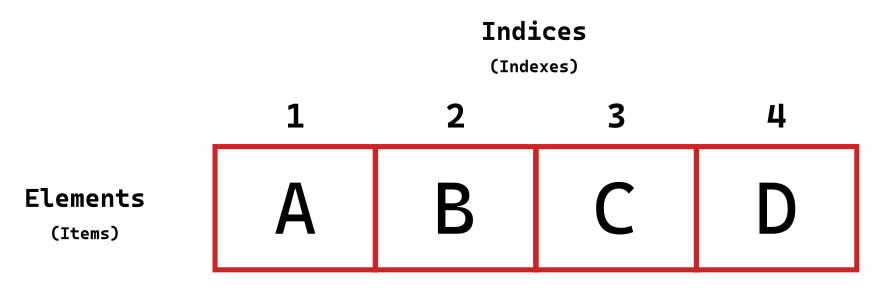
\includegraphics[width=0.8\textwidth]{arrays.png}
    \caption{A breakdown and representation of an array.}
    \label{fig:arrays}
\end{figure}

In figure \ref{fig:arrays}, the index is the nth element. Indices in other languages like Python begin at 0, and for a very good reason\footnote{Advanced learners: this is due to its heritage in older languages like C. Arrays are actually not values that stand by themselves, as the size isnt promised to be some value. Attempting to remove/modify the array will cause memory to overlap, which is very bad. Instead, an array is simply a \emph{location in memory where data is}. The location in memory will have the array's data; uniformly sized data that are equally spaced out. Therefore, if you were to get the first item of a list at address 4000, the first item would be 4000+0. However, the second one would be 1 address away, so 4000+1, then 4000+2, etc. This is why arrays begin at 0; it is simply the \emph{offset} from the beginning of the memory address.}. However, you just need to remember that indices start at 1 in pseudocode.

To index that array (let's call it {\ccmono Array}), one may write {\ccmono Array[<index>]}. In code, it looks like

\begin{minted}{text}
OUTPUT Array[2] // gets the second item in the array.
\end{minted}

In fact, you may also write to the array this way:

\begin{minted}{text}
Array[2] <- 'F' // sets the second element to the character F.
\end{minted}

To wrap this new knowledge up, let us create an array of food items.

\begin{minted}{text}
DECLARE FoodItems:ARRAY[1:5] OF STRING
\end{minted}

We must fill it up with items. In programming terms, this is known as \emph{populating}.

\begin{minted}{text}
FoodItems[1] <- "Burger"
FoodItems[2] <- "Chilli Crab"
FoodItems[3] <- "Paneer Tikka"
FoodItems[4] <- "Fried Rice"
FoodItems[5] <- "Beans on Toast"
\end{minted}

Now, there are items in the list and we can freely index it now!

\subsubsection{Iterating through an array}

Revisit section \ref{sec:for_loops} on for loops.

\begin{minted}{text}
FOR Counter <- 1 TO 5
    OUTPUT Counter
NEXT Counter
\end{minted}

For loops allow us to count through values between 1 and something. Conveniently, array indexes are numbers. \textbf{Do you see the pattern?}

\textbf{YES! We can use for loops to go through the items in a list!}

\begin{minted}{text}
FOR Counter <- 1 TO 5 // our list is 5 items long
    OUTPUT FoodItems[Counter]
NEXT Counter
\end{minted}

Will output:

\begin{minted}{text}
Burger
Chilli Crab
Paneer Tikka
Fried Rice
Beans on Toast
\end{minted}

Armed with this information, let us practice.

\newpage
\subsubsection{Exercises}
\label{ex:3_2_3}

Write pseudocode for all below questions.

\begin{enumerate}
    \item With the array we declared before, loop through it backwards and print {\ccmono Do you like <the food item>?}
        \mediumlines
    \item Create a constant {\ccmono FoodsLength} and set it to 10. Create a new array {\ccmono FoodsLength} items long called {\ccmono FavoriteFoods}.
        \mediumlines
    \item Move all the items in the old array to the new array, without copying the values directly. Only use indexing to move the values.
        \mediumlines
    \item Redo question 3, but you may not write more than 3 lines. Use the correct loop for this.
        \mediumlines
    \item In the most logical and optimized manner, ask the user to populate the 6th to the 10th index in the new array through user input and a loop of your choosing. Do not write more than 1 input statement. \emph{hint: counters and indexing!}
        \largelines
    \item Iterate through your new list and print out each of the items in the list. 
        \largelines
\end{enumerate}

\newpage
\subsection{2D arrays}

2D arrays are not dissimilar from plain 1D arrays. In essence, they are still arrays; and the primitive definition of a 2D array would be an array of arrays.

\begin{figure}[h]
    \centering
    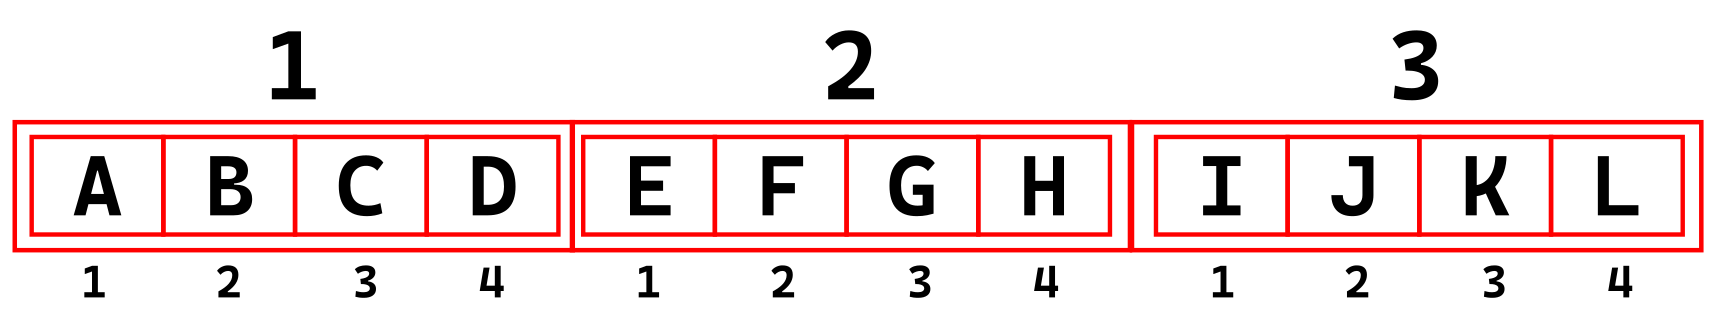
\includegraphics[width=0.95\textwidth]{2darray.png}
    \caption{A (bad) visual representation of a 1D array.}
    \label{fig:2darray}
\end{figure}

Declaring them can be done as follows:

\begin{minted}{text}
//                         COLUMNS       ROWS
DECLARE <variable>:ARRAY[<begin>:<end>,<begin>:<end>] OF <type>
\end{minted}

Confusing, right?

In this sense, 2D arrays will not be very useful. Arrays in arrays, pretty ridiculous, right?

But no, imagine a situation where you are using an array of names to represent peoples' lockers, and you store the name of each student.

\begin{figure}[h]
    \centering
    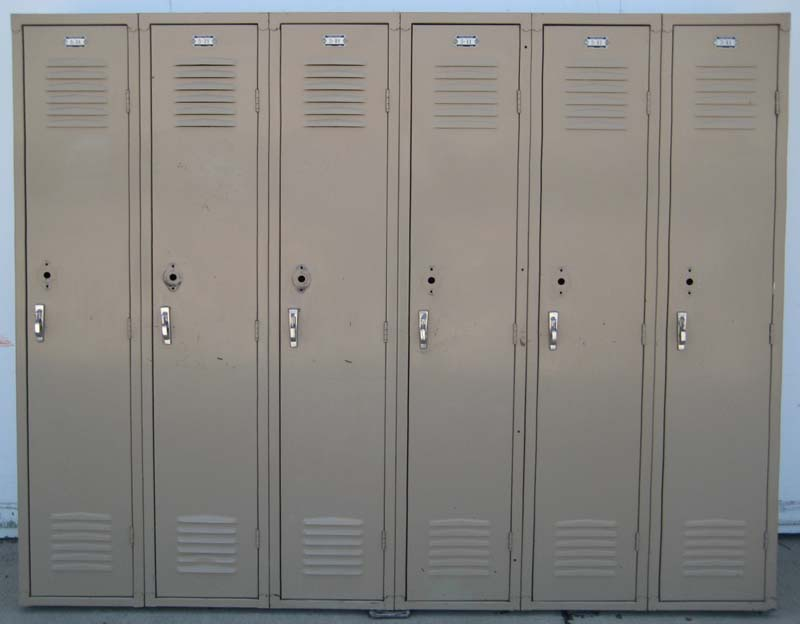
\includegraphics[width=0.6\textwidth]{lockers.jpg}
    \caption{American High School Lockers.}
    \label{fig:lockers}
\end{figure}

(Lockers are to be imagined as the ones depicted in figure \ref{fig:lockers}.)

However, imagine if your school replaced the lockers with the ones similar to the ones at our school. Instead of being a linear list of lockers, it would be more like a grid, 3 lockers high. Now you need to store the names of the students for the lockers; what do you do?

The smart solution would be to store the names in a list for a row, and store 3 rows in a list itself. Boom, 2D array!

\begin{figure}[h]
    \centering
    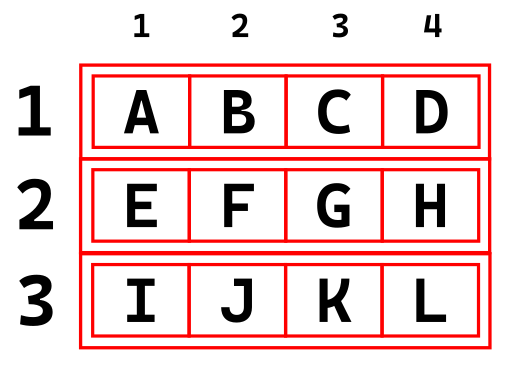
\includegraphics[width=0.6\textwidth]{2darray_matrix.png}
    \caption{2D arrays represented with a matrix.}
    \label{fig:2darray_matrix}
\end{figure}

The objective of my explanation is not to explain why 2D arrays are so useful for lockers. It's that 2D arrays give you matrix superpowers in your code; suddenly you can store tables and grids in your code. From a tic tac toe\footnote{Noughts and Crosses for those who are in/from the UK!} board, to battleships; lockers, apartments and even student scores (foreshadowing), 2D arrays gives you a lot of opportunities.

\subsubsection{Declaration and Population}

Let us declare the 2D array we described.

\begin{minted}{text}
DECLARE Lockers:ARRAY[1:8,1:3] OF STRING
\end{minted}

Indexing a 2D array is as simple as providing 2 indexes. The first of which is the row, and the second of which is the column. This may seem very, very counterintuitive, but looking back at figure \ref{fig:2darray}, 2D arrays are stored rows-first, so to access a cell in the grid, you must get the correct row first. This is contrary to math, where coordinates on the cartesian plane are specified as {\ccmono (x, y)}, such as {\ccmono (5, 2)}. To get the cell at {\ccmono (5, 2)} in math terms, we write:

\begin{minted}{text}
OUTPUT Lockers[2,5]
\end{minted}

And to populate it, we do a very similar thing to a 1D array.

\begin{minted}{text}
Lockers[2,5] <- "Jonathan"

// et cetera, fill it up however you require.
\end{minted}

\subsubsection{Iteration}

Remember when we used a single for loop to loop through a 1D array? Now, guess what you do to iterate through a 2D array.

...if you guessed a nested loop, you are correct. The inner loop here would loop through one row, and the outer loop controls how many rows are iterated through.

\begin{minted}{text}
DECLARE CurrentName:STRING
CurrentName <- "" // it is always good practice to initialize your
                   // variable after you declare it!

FOR Row <- 1 TO 3
    FOR Column <- 1 TO 8
        CurrentName <- Lockers[Row,Column]

        OUTPUT "The student at row ", Row, " column ",
               Column "'s name is", CurrentName
    NEXT Column

    OUTPUT "Done with row ", Row
NEXT Row
\end{minted}

The code example is complicated but it is straightforward when you read it very carefully:

\begin{itemize}
    \item The first 2 lines declares and initializes a variable to make life easier.
    \item Line 4 begins a loop that loops through the 3 rows we declared.
    \item Line 5 begins a loop \emph{inside} the previous loop that goes through each column.
    \item We use the variable on line 6 so we dont have to type {\ccmono Lockers[Row,Column]} in the output line. As mentioned previously, it simplifies the task.
    \item Line 8 looks intimidating, but it just formats the string so it looks something like, {\ccmono The student at row 2 column 5's name is Jonathan}.
    \item Line 11 prints out some text to indicate the row is done.
\end{itemize}

This is a very challenging topic; but if you made it this far; give yourself a pat on the back (or ask your friend :))

Exercises next; they will not get easier than before :)

\newpage
\subsubsection{Exercises}
\label{ex:3_3_3}

As usual, write all questions in pseudocode.

\begin{enumerate}
    \item Modify the code block above to loop through the rows and columns backwards. Simply state the lines that need to be rewritten.
        \smalllines
    \item Declare a 5x5 2D array to store students' exam scores, betewen 0 and 100. Choose the correct data type.
        \smalllines
    \item Justify why you picked the type you picked for question 2. Include the boundaries/the type of data the data type supports.
        \mediumlines
    \item Ask the user to populate each cell. Tell the user which cell they are populating. Only allow numbers between 5 and 10 to be input into the table. Else, tell the user to tell again and do so until the number is between 5 and 10.
        \verylargelines
\end{enumerate}

\newpage
\subsection{Parallel Arrays (2D arrays)}

This is a short section explaing what parallel arrays are.

The naïve definition of parallel arrays are arrays that go in parallel, one index are associates with another.

Unclear, right?

Now imagine this dataset:

\begin{itemize}
    \item I have a list of names ({\ccmono DECLARE ARRAY[1:5] OF STRING}).
    \item I have a bunch of exam scores that correspond to the students in the array. Each student has 3 exam scores for Science, Math and English.
\end{itemize}

Judging by the activity we just did, can you guess how we can store the scores? Yes! a 2D array. Since the 3 exam scores are repeating for each student, we can have a 2D array like the following:

\begin{figure}[ht]
    \centering
    \begin{tabular}{ |c|c|c|c| }
        \hline 
        \textbf{Index} & 1 & 2  & 3  \\ \cline{2-4}
              & \textbf{Science} & \textbf{Math} & \textbf{English} \\ \hline
        1     & 90      & 95   & 70 \\ \hline
        2     & 80      & 80   & 90 \\ \hline
        3     & 65      & 75   & 80 \\ \hline 
        4     & 25      & 30   & 30 \\ \hline
        5     & 100     & 65   & 80 \\ \hline
    \end{tabular}
    \caption{The data set in question. We will call it {\ccmono StudentScores}}.
    \label{tab:scores_dataset}
\end{figure}

and student names in a normal array. Then, you can have a setup as follows:

\begin{figure}[h]
    \centering
    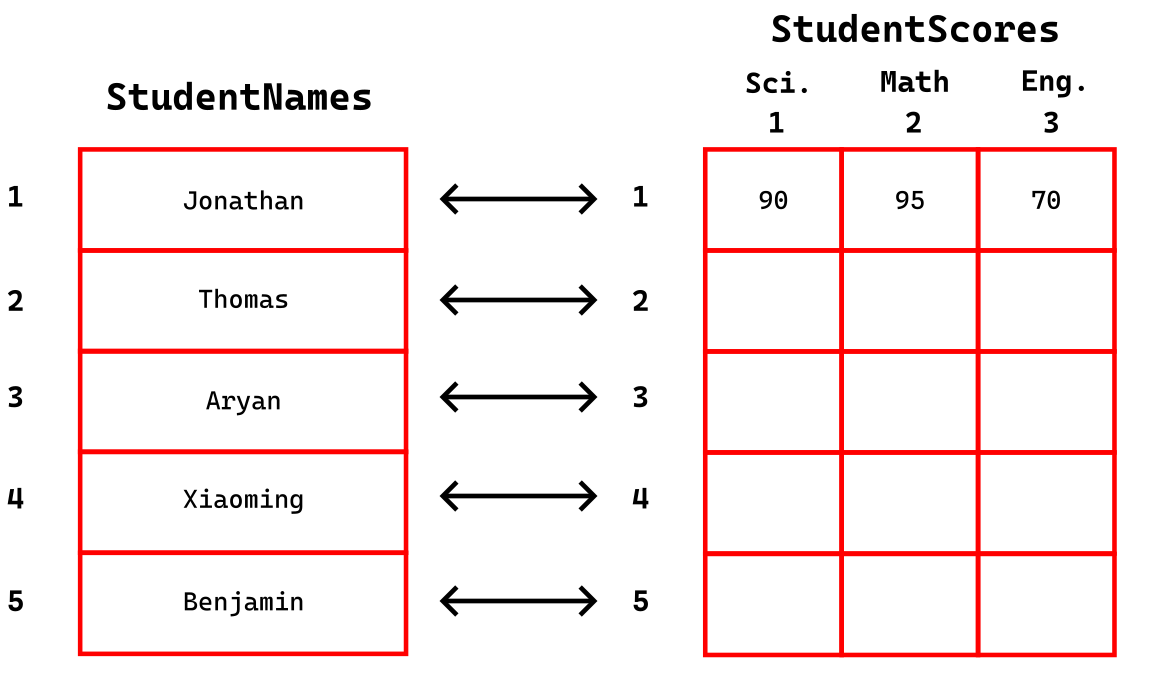
\includegraphics[width=0.7\textwidth]{parallel_arrays.png}
    \caption{parallel arrays.}
    \label{fig:parallel_arrays}
\end{figure}

Figure \ref{fig:parallel_arrays} shows the data (unfortunately truncated, as I do not want to copy all the data in) in terms of parallel arrays. Now, you may be able to see the etymology; parallel refers to the nature of the arrays where each of the arrays are correlated by the index. You can simply \emph{define} and even assert that whichever name you insert into the names array, the right must correspond to the results. Therefore, when writing code, you can use the index to bind the arrays together in some regard; they suddenly become related and associated by the index and you now have 2 arrays in parallel by which you can store complex data.

In terms of code, this means you could, say print the names and scores together, calculate the average score and manipulate the name string all while the data is tied together, In fact,

\subsubsection{Exercises}
\label{ex:3_4_1}

As always, write all below answers in pseudocode.

\begin{enumerate}
    \item Write code to print out the parallel arrays. Output the name of the student and their corresponding scores.
        \verylargelines
    \item Write code to print out the student's name, but this time, the average of their scores as well.
        \verylargelines
    \item Write code to determine who has the lowest average in the class. You may keep an extra variable and conditionally set it somehow. Print out the lowest scoring student's name and average at the end.
        \verylargelines
    \item \textbf{Yay! No more exercises..from me. Do the last question of a Comp Sci past paper 2 from recently; ask your computer science teacher for a copy (you should already have one) :)}
\end{enumerate}

\end{document}
